% Holmes 论文精读笔记 —— notebrick 风格
% 编译：xelatex main.tex （运行两遍以生成目录与总页码）
\documentclass[11pt,a4paper,UTF8,fontset=windows]{ctexart}

% ---------- 页面 ----------
\usepackage[a4paper,top=2.55cm,bottom=2.75cm,left=2.35cm,right=2.35cm,headheight=22pt]{geometry}
\usepackage{amsmath,amssymb,mathtools}
\usepackage{graphicx}
\usepackage{booktabs}
\usepackage{multirow}
\usepackage{xcolor}
\usepackage[most,breakable]{tcolorbox}
\usepackage{enumitem}
\usepackage{caption}
\usepackage{fancyhdr}
\usepackage[colorlinks=true,linkcolor=linkblue,urlcolor=linkblue,citecolor=linkblue]{hyperref}

% ---------- 颜色 ----------
\definecolor{structbg}{HTML}{EFF4FA}   % 结构与模型框底色（淡蓝）
\definecolor{structframe}{HTML}{8FA8C4}
\definecolor{structtitle}{HTML}{1F4E79}
\definecolor{thinkbg}{HTML}{FAF4E7}   % 思考框底色（米色）
\definecolor{thinkframe}{HTML}{CE9A78}
\definecolor{thinktitle}{HTML}{8C4A2F}
\definecolor{greybg}{HTML}{F3F3F3}    % 补充/复现框底色（浅灰）
\definecolor{greyframe}{HTML}{B0B0B0}
\definecolor{greytitle}{HTML}{454545}
\definecolor{linkblue}{HTML}{1F4E79}
\definecolor{inkgray}{HTML}{86868B}

% ---------- 版式 ----------
\ctexset{
  section = {format={\heiti\zihao{3}\color{ink}}, beforeskip=1.6ex plus .2ex, afterskip=1.1ex,
             number={\arabic{section}}, name={,　}},
  subsection = {format={\heiti\bfseries\zihao{4}\color{ink}}, beforeskip=1.2ex plus .2ex, afterskip=0.8ex,
             number={\arabic{section}.\arabic{subsection}}, name={,　}},
}
\definecolor{ink}{HTML}{1D1D1F}

% 目录带点线（section 与 subsection 一致）
\makeatletter
\renewcommand*\l@section{\@dottedtocline{1}{0em}{2.3em}}
\makeatother

% 页眉页脚
\pagestyle{fancy}
\fancyhf{}
\fancyhead[L]{\zihao{-5}\color{inkgray}论文精读笔记}
\fancyhead[R]{\zihao{-5}\color{inkgray}Holmes · ICML 2026}
\fancyfoot[C]{\zihao{-5}\color{ink}\thepage\ /\ \pageref{LastPage}}
\renewcommand{\headrulewidth}{0.4pt}
\renewcommand{\headrule}{\hbox to\headwidth{\color{inkgray}\leaders\hrule height \headrulewidth\hfill}}

% ---------- 代码与词条 ----------
\newcommand{\code}[1]{\texttt{#1}}
\newcommand{\term}[1]{\textbf{#1}}

% ---------- 盒子 ----------
% 结构与模型 N：淡蓝
\newtcolorbox[auto counter]{structbox}[2][]{
  breakable, enhanced,
  colback=structbg, colframe=structframe,
  boxrule=0.7pt, arc=1.6mm, left=8pt, right=8pt, top=7pt, bottom=7pt,
  toptitle=3pt, titlerule=0pt,
  title={\heiti\color{structtitle}结构与模型\quad\thetcbcounter\quad #2},
  coltitle=structtitle, fonttitle=\normalsize,
  attach boxed title to top left={xshift=6pt, yshift=-\tcboxedtitleheight/2},
  boxed title style={colback=structbg, frame hidden, boxrule=0pt},
  #1
}
% 思考：米色
\newtcolorbox{thinkbox}[1][]{
  breakable, enhanced,
  colback=thinkbg, colframe=thinkframe,
  boxrule=0.7pt, arc=1.6mm, left=8pt, right=8pt, top=7pt, bottom=7pt,
  toptitle=3pt, titlerule=0pt,
  title={\heiti\color{thinktitle}思考\quad #1},
  coltitle=thinktitle, fonttitle=\normalsize,
  attach boxed title to top left={xshift=6pt, yshift=-\tcboxedtitleheight/2},
  boxed title style={colback=thinkbg, frame hidden, boxrule=0pt}
}
% 补充：浅灰
\newtcolorbox{greybox}[2][]{
  breakable, enhanced,
  colback=greybg, colframe=greyframe,
  boxrule=0.7pt, arc=1.6mm, left=8pt, right=8pt, top=7pt, bottom=7pt,
  toptitle=3pt, titlerule=0pt,
  title={\heiti\color{greytitle}#2},
  coltitle=greytitle, fonttitle=\normalsize,
  attach boxed title to top left={xshift=6pt, yshift=-\tcboxedtitleheight/2},
  boxed title style={colback=greybg, frame hidden, boxrule=0pt},
  #1
}

\captionsetup{font=small, labelfont={bf}, labelsep=quad}
\setlength{\parskip}{0.35em}

% 数学算子
\DeclareMathOperator*{\argmax}{arg\,max}
\newcommand{\vect}[1]{\boldsymbol{#1}}

\begin{document}

% ================= 封面 =================
\thispagestyle{fancy}
\begin{center}
  {\heiti\zihao{2}\color{ink}Holmes 论文精读笔记}\\[1.1em]
  {\zihao{-3}\color{inkgray}Revisiting Uncertainty: On Evidential Learning for Partially Relevant Video Retrieval}\\[0.7em]
  {\zihao{-4}\color{inkgray}ICML 2026\quad·\quad 部分相关视频检索（PRVR）\quad·\quad 证据式深度学习}\\[1.4em]
  {\zihao{-4}\color{inkgray}2026 年 11 月 16 日}
\end{center}
\vspace{0.4em}

\tableofcontents
\vspace{0.4em}

\noindent 这篇笔记把 Holmes 从头到尾精读一遍，供组会 pre 使用。行文按“信息与概括 $\rightarrow$ 背景与动机 $\rightarrow$ 证据式学习预备 $\rightarrow$ 方法 $\rightarrow$ 实验 $\rightarrow$ 代码 $\rightarrow$ 批判性思考”的顺序展开；所有关键公式都按论文编号重排成结构框，方便 pre 时直接照着推。读每一步都建议抓三件事：\term{它解决什么问题}，\term{它的计算怎么做}，以及\term{它和相邻方法的区别在哪里}。最后一章专门整理了 pre 时可能被问到的问题和参考回答。

% ================= 1 论文信息与概括 =================
\section{论文信息与一句话概括}

\subsection{基本信息}

\begin{table}[h]
\centering
\small
\begin{tabular}{@{}ll@{}}
\toprule
标题 & Revisiting Uncertainty: On Evidential Learning for Partially Relevant Video Retrieval \\
作者 & Jun Li, Peifeng Lai, Xuhang Lou, Jinpeng Wang, Yuting Wang, Ke Chen, Yaowei Wang, Shu-Tao Xia \\
机构 & 清华大学深圳国际研究生院；鹏城实验室；哈尔滨工业大学（深圳） \\
会议 & ICML 2026（PMLR 306，首尔） \\
论文 & \url{https://arxiv.org/abs/2605.06083} \\
官方代码 & \url{https://github.com/lijun2005/ICML26-Holmes}（已 fork 至 \url{https://github.com/gry1024/ICML26-Holmes}） \\
中文解读 & 52CV 公众号；作者系列工作 HLFormer（ICCV 25）、DreamPRVR（CVPR 26）、Awesome-PRVR \\
\bottomrule
\end{tabular}
\end{table}

\subsection{一句话概括}

PRVR（Partially Relevant Video Retrieval）要用\term{只描述局部内容的短查询}检索未裁剪长视频，天然存在不确定性。Holmes 把检索过程中的“相似度分数”重新解释为\term{证据}，用 Dirichlet 分布对查询的不确定性做显式建模：在\term{视频之间}（inter-video）识别出精确／多义／欠定三类查询并做自适应标签校准，在\term{视频内部}（intra-video）用带“尘桶”（dustbin）的灵活最优传输把查询软对齐到多个相关片段，从而同时缓解语义歧义与稀疏监督。三个基准上 SumR 全面领先：ActivityNet Captions \textbf{156.8}、Charades-STA \textbf{80.6}、TVR \textbf{198.6}。

\medskip
\noindent 论文自述的三条贡献：
\begin{enumerate}[itemsep=1pt,topsep=2pt]
  \item \term{概念层}：首次把 PRVR 的问题统一到“不确定性”视角下，把视频间语义歧义与视频内稀疏监督显式关联起来；
  \item \term{方法层}：提出层次化证据学习框架 Holmes，含三重准则（epistemic uncertainty、label consistency、aleatoric uncertainty）驱动的细粒度查询识别与标签校准，以及带自适应尘桶的灵活最优传输（FOT）实现稠密且鲁棒的时序对齐；
  \item \term{实验层}：三大基准 SOTA，消融与可视化证明其能量化查询歧义、抑制 MIL 引起的虚假局部激活。
\end{enumerate}

% ================= 2 背景与动机 =================
\section{背景：任务与两大挑战}

\subsection{任务定义：PRVR}

给定文本查询 $T$，要求从未裁剪的视频库 $\mathcal{V}$ 中排序并返回\term{包含相关瞬间的视频}。与三类近邻任务的区别要能说清楚：
\begin{itemize}[itemsep=1pt,topsep=2pt]
  \item \term{T2VR}（文本到视频检索）：视频是预裁剪的，查询完整描述全部内容——假设在真实场景并不成立；
  \item \term{VCMR}（视频库瞬间检索）：除了视频级检索还要定位瞬间，需要瞬间级标注，可扩展性差；
  \item \term{PRVR}：视频未裁剪、查询只对应其中一小段，只在\term{视频级}标注“哪个视频与这条查询相关”，不要求瞬间级标注。
\end{itemize}

这种“短查询 vs.\ 长视频”的\term{数据不对称}是全篇的出发点：查询通常简短而含糊，视频内容丰富而冗长，检索过程必然引入不确定性。

\subsection{挑战一：视频间语义歧义}

真实查询存在细粒度异质性。论文用四类真实样本说明（见原文 Figure 1）：
\begin{itemize}[itemsep=1pt,topsep=2pt]
  \item \term{精确查询}（precise）：如 “He pulls the man from the river by car.”——GT 视频与候选之间有清晰的响应间隔，检索可靠；
  \item \term{欠定查询}（under-determined）：如 “An athlete flexes his guns.”——语义不足，模型“看不懂查询”，对各候选的响应弱且无区分度，置信度低；
  \item \term{多义查询}（polysemous）两种情形：“A person is shoveling the driveway.”（GT 是对的但不确定，多个语义相近的候选都得到高响应）与 “The man spins and releases.”（一句话匹配多个合理视频）——需要\term{更多斟酌}来处理关联的不确定性。
\end{itemize}

既有方法要么完全忽略这种异质性（GMMFormer 等），要么用正则化隐式处理（RAL、MSC-PRVR），要么只检测“歧义对”而不量化歧义类型（ARL）。Holmes 的立场是：应该\term{显式地量化不确定性的类型与大小}，再据此调整监督信号。

\subsection{挑战二：视频内稀疏监督}

主流的 MIL（多示例学习）范式只用\term{单个最佳匹配片段}计算损失：$s_f=\max_i \cos(\vect q,\vect f_i)$。这带来两个问题：
\begin{enumerate}[itemsep=1pt,topsep=2pt]
  \item \term{监督稀疏}：每个“查询–视频”正样本对只有 $1$ 个片段位置获得梯度，其余片段训练不足（under-trained），模型学不到整体表示；
  \item \term{虚假尖峰}：欠训练的片段容易被全局无关内容激活。原文例子：查询 “The girl bends down and ties the ballerina shoes.”，一个内容为 running 的无关视频在某个 token 上打出 $\max=0.682$ 的尖峰分数，超过 GT 视频的 $0.435$，直接导致检索失败。
\end{enumerate}

用 CLIP 蒸馏可以补充稠密信号（DL-DKD），但帧级片段缺乏时序动态，无法真正“确认视频相关”，反而加剧视频间的不确定性。论文的判断是：两个挑战\term{互为因果}——视频内证据不足会放大视频间歧义，因此需要一个统一框架在两个层级同时积累证据。

\begin{thinkbox}[为什么是“证据”而不是“分数”？]
确定性打分模型只回答“多像”，不回答“我多有把握”。当查询本身含糊、视频内证据又稀疏时，一个高的相似度可能是真匹配，也可能是噪声尖峰——单点分数无法区分两者。证据式学习把每次匹配看作对某个假设的支持度积累，天然带有“信念质量”与“不确定质量”两个出口，这正是区分四类查询、决定“该信多少标签”所需要的中间量。
\end{thinkbox}

\subsection{相关工作脉络}

\begin{table}[h]
\centering
\small
\begin{tabular}{@{}llll@{}}
\toprule
方法 & 出处 & 核心思路 & 对不确定性的处理 \\
\midrule
MS-SL & MM 2022 & 提出任务；滑窗冗余片段嵌入 + MIL & 无 \\
DL-DKD & ICCV 2023 & CLIP 知识蒸馏补稠密信号 & 无（帧级片段加剧歧义） \\
GMMFormer(V2) & AAAI 24/25 & 高斯注意力隐式建片段 & 无 \\
ProtoPRVR & AAAI 2025 & 原型片段加速检索 & 无 \\
RAL & 2025 & 概率嵌入 + 正则 & 隐式（正则化） \\
MSC-PRVR & 2025 & 辅助损失缓解语义坍缩 & 隐式 \\
ARL & AAAI 2025 & 显式检测歧义“对” & 只判“是否歧义”，无类型量化 \\
HLFormer / DreamPRVR & ICCV 25 / CVPR 26 & 作者前作：层级结构与生成式表示 & 无显式不确定性 \\
\midrule
\term{Holmes} & ICML 2026 & 层次化证据学习（Dirichlet + OT） & \term{显式三分类 + 标签校准 + 软对齐} \\
\bottomrule
\end{tabular}
\caption{PRVR 代表方法与 Holmes 的定位。}
\end{table}

% ================= 3 预备知识 =================
\section{预备知识：证据式深度学习（EDL）}

EDL（Sensoy et al., 2018）源自 Dempster--Shafer 证据理论与主观逻辑（Subjective Logic），核心是把分类问题从“输出一个概率向量”升级为“输出对 $K$ 个类别的\term{证据量}，再由证据诱导二阶分布”。

\begin{structbox}{Dirichlet 参数化与主观逻辑量}
设查询 $q_i$ 对 $K$ 个候选视频的相似度为 $s_{ij}$。按以下链条把分数变成证据、再变成信念：
\begin{align}
e_{ij} &= \exp\!\big(\tanh (s_{ij}/\tau)\big), \qquad \vect e_i = [e_{i1},\dots,e_{iK}], \label{eq:evidence}\\
\alpha_{ij} &= e_{ij} + 1, \qquad S_i = \sum_{j=1}^{K} \alpha_{ij}, \label{eq:alpha}\\
b_{ij} &= \frac{\alpha_{ij}-1}{S_i} \quad(\text{信念质量}), \qquad u_i = \frac{K}{S_i} \quad(\text{认知不确定度}), \label{eq:belief}
\end{align}
满足 $u_i + \sum_j b_{ij} = 1$：信念与不确定度瓜分单位质量。$\vect\alpha_i$ 是 Dirichlet 分布 $\mathrm{Dir}(\vect p;\vect\alpha_i)$ 的浓度参数，$S_i$ 越大，分布越尖锐、不确定度 $u_i$ 越小。
\end{structbox}

\begin{greybox}{补充　为什么是 Dirichlet 而不是 softmax}
softmax 给出 $\vect p$ 的点估计，不确定性只能靠温度或多次前向近似。Dirichlet 是\term{定义在概率单纯形上的分布}（分布之上的分布），它的期望 $\mathbb{E}[p_k]=\alpha_k/S$ 给出点估计的同时，还用 $S$（强度）刻画“这个估计有多可信”，一次前向即得两类不确定性（认知 $u$ 与偶然 $\xi$，见后），无需采样。这是 Holmes 能零开销地做不确定性建模的根基——论文效率实验显示其开销与不含证据模块的 GMMFormerV2 基本持平。
\end{greybox}

\begin{thinkbox}[与贝叶斯网络 / MC Dropout 的对比]
BNN 与 MC Dropout 都要多次前向或改架构，且只给出笼统的“模型不确定性”，难以区分“查询本身含糊”还是“证据不足”。EDL 的主观逻辑分解天然给出两个出口：$u_i$（证据总量不足）与 $\xi_i$（证据在候选间分散，见 \eqref{eq:aleatoric}），恰好对应欠定与多义两类查询——这是三重准则得以成立的前提。
\end{thinkbox}

% ================= 4 方法 =================
\section{方法：Holmes 框架}

\subsection{总览与基础组件}

\begin{figure}[h]
\centering
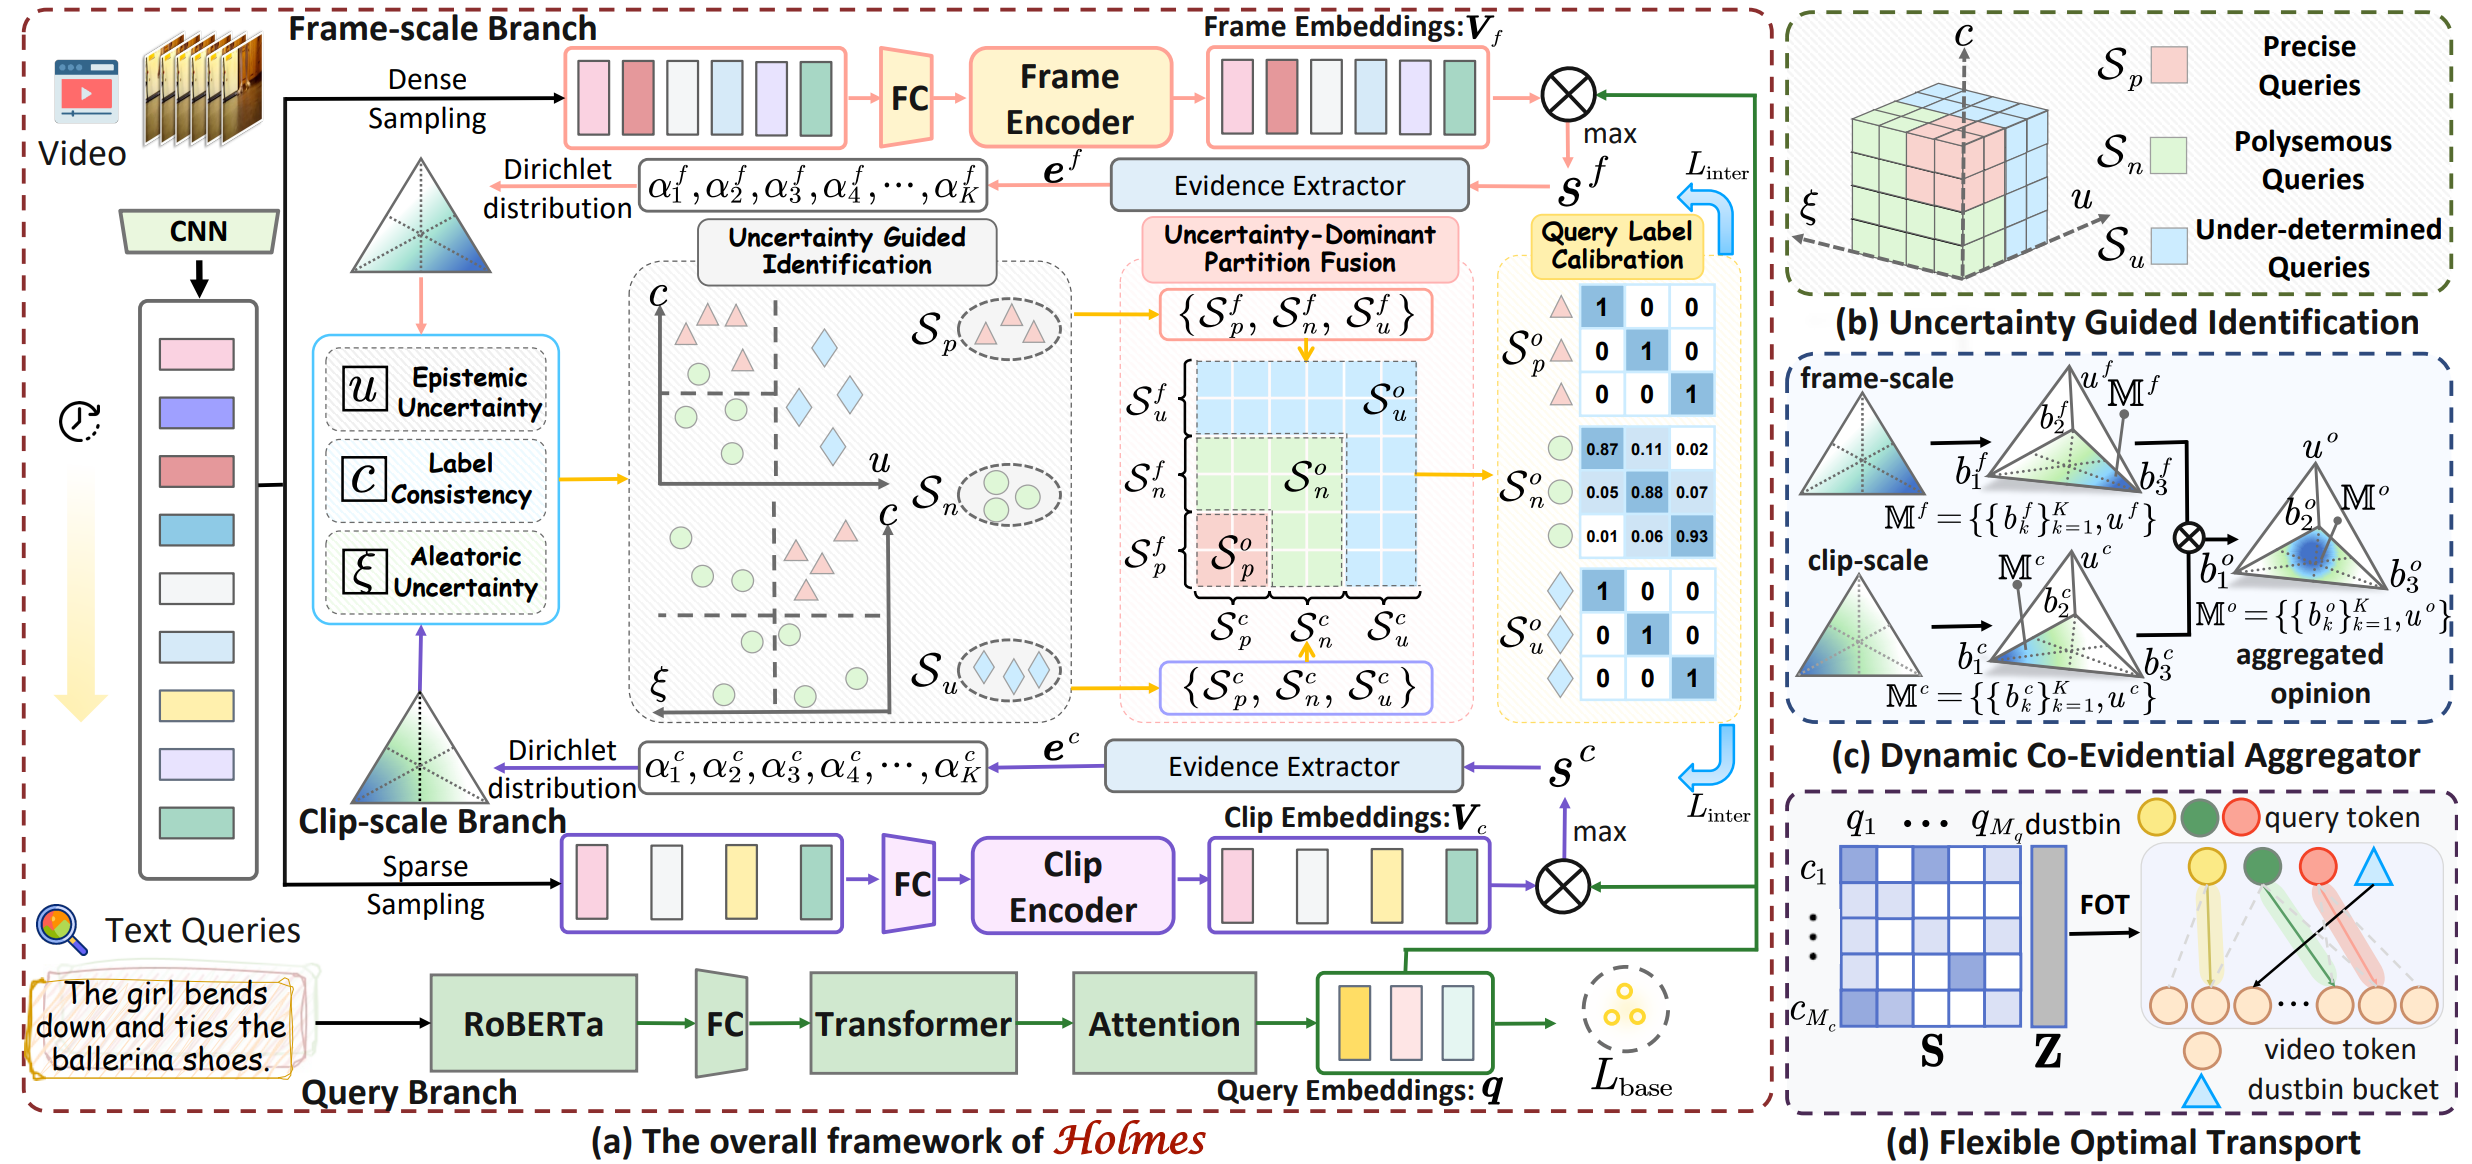
\includegraphics[width=\linewidth]{holmes_framework.png}
\caption{Holmes 总体框架（摘自官方仓库）。查询分支输出 $\vect q$；帧／片段双分支提取 $\vect V_f,\vect V_c$；候选相似度转为证据向量并用 Dirichlet 建模，据三重准则做不确定性引导的识别（UGI），双尺度划分经不确定性主导的分区融合（UDPF）得到最终 $S^o_p,S^o_n,S^o_u$；查询标签校准后由 $\mathcal{L}_{\mathrm{inter}}$ 监督；视频内用带尘桶的 FOT 建立软查询–片段指派，作为 $\mathcal{L}_{\mathrm{intra}}$ 的标签证据。}
\end{figure}

\begin{structbox}{双分支视频表示与相似度}
文本侧：预训练 RoBERTa + 投影层 + Transformer，注意力池化为 $\vect q\in\mathbb{R}^d$（同 MS-SL）。视频侧双分支：
帧分支把 $M_f$ 个采样帧经 FC 与帧编码器得 $\vect V_f=\{\vect f_i\}_{i=1}^{M_f}$；片段分支把视频稀疏切成 $M_c$ 个片段，经投影与片段编码器得 $\vect V_c=\{\vect c_i\}_{i=1}^{M_c}$。两个尺度的相似度与总分：
\begin{align}
s_f(T,V) &= \max\{\cos(\vect q,\vect f_1),\dots,\cos(\vect q,\vect f_{M_f})\},\qquad
s_c(T,V) \ \text{同理}, \label{eq:sim}\\
s(T,V) &= \alpha_f\, s_f(T,V) + \alpha_c\, s_c(T,V),\qquad \alpha_f+\alpha_c=1. \label{eq:totalsim}
\end{align}
检索与排序只依赖 \eqref{eq:totalsim}。TVR 配置中 $\alpha_f=0.4$、$\alpha_c=0.6$（见 \code{clip\_scale\_w}）。
\end{structbox}

注意一个关键设计：双分支\term{不是}简单的特征融合，而是\term{两个独立的证据源}——各自跑完整的 inter-video 证据学习，最后用 DST 规则融合（见 \S\ref{sec:aggregator}）。

\subsection{Inter-video 证据学习}

\subsubsection{三重准则}

只用 $u_i$ 不够。论文给出两个“否定式”结论作为动机（原文 Theorem 3.2 与 Proposition 3.4）：
\begin{align}
\text{低 } u_i \ \not\Rightarrow\ \arg\max_j b_{ij} = \arg\max_j y_{ij}
\quad\text{（证据多，但可能押错视频）；}\qquad
\text{高 } c_i \ \not\Rightarrow\ \text{查询精确}
\quad\text{（GT 响应高，别的候选也可能一样高）}.
\end{align}
Theorem 3.2 的证明是构造性的反例：把全部证据 $\lambda$ 押在一个错误视频 $k$ 上，则 $u_i=K/(\lambda+K)\to 0$（任意低），但最高信念落在 $k\neq t$。因此需要三个量配合：

\begin{structbox}{三重准则}
对查询 $q_i$（$\vect y_i$ 为 one-hot 标注，$\vect s_i$ 为对 $K$ 个候选的相似度）：
\begin{align}
&\text{认知不确定度（epistemic）：}\quad u_i = \frac{K}{S_i}, \label{eq:epistemic}\\
&\text{标签一致性（label consistency）：}\quad c_i = \max\big(0,\ \vect s_i\cdot\vect y_i\big), \label{eq:consistency}\\
&\text{偶然不确定度（aleatoric）：}\quad
\xi_i = \mathbb{E}_{\vect p\sim\mathrm{Dir}(\vect\alpha_i)}[H(\vect p)]
= \sum_{k=1}^{K}\frac{\alpha_{ik}}{S_i}\Big(\psi(S_i+1)-\psi(\alpha_{ik}+1)\Big), \label{eq:aleatoric}
\end{align}
其中 $\psi$ 为 digamma 函数。$u$ 高 $\Leftrightarrow$ 证据总量少（欠定）；$c$ 低 $\Leftrightarrow$ GT 响应弱；$\xi$ 高 $\Leftrightarrow$ 概率质量分散在多个候选（多义），$\xi$ 低 $\Leftrightarrow$ 质量集中于单个视频（精确）。
\end{structbox}

三个量各管一段，形成完整的判别链：$u$ 先筛掉“看不懂的”，$c$ 再看“押没押对”，$\xi$ 最后区分“唯一可靠”与“多个都像”。

\subsubsection{不确定性引导的识别（UGI）}

\begin{structbox}{三分类与自适应阈值}
以正确匹配对集合 $S_{\mathrm{tp}}=\{i \mid \arg\max(\vect s_i)=\arg\max(\vect y_i)\}$ 为锚点，取
\begin{align}
\beta_u = \min\!\big(u_{\mathrm{tp}},\ 1-\beta\big),\qquad
\beta_p = \max\!\big(\beta,\ c_{\mathrm{tp}}\big),\qquad \beta = 0.3,
\end{align}
其中 $u_{\mathrm{tp}}=\max_{i\in S_{\mathrm{tp}}} u_i$、$c_{\mathrm{tp}}=\min_{i\in S_{\mathrm{tp}}} c_i$。据此三分类：
\begin{align}
S_u &= \{q_i \mid u_i > \beta_u\} \quad(\text{欠定})，\\
\tilde S_p &= \{q_i \mid u_i \le \beta_u,\ c_i \ge \beta_p\} \quad(\text{初步精确})，\\
\tilde S_n &= \{q_i \mid u_i \le \beta_u,\ c_i < \beta_p\} \quad(\text{初步多义}).
\end{align}
由于 $\tilde S_p$ 中仍混有多义查询（Proposition 3.4），再按 $\xi$ 以中位数细分：
\begin{align}
S_p = \{q_i\in\tilde S_p \mid \xi_i < \mathrm{median}\{\xi_j\}_{q_j\in \tilde S_p}\},\qquad
S_n = (\tilde S_p\cup\tilde S_n)\setminus S_p .
\end{align}
\end{structbox}

阈值不拍脑袋：以\term{当前模型已检索正确的样本}的不确定度包络为锚，保证“精确”的标准不高于模型自身的可靠水平；$\beta=0.3$ 只做安全垫。消融显示用固定阈值或只用 $\tilde S_n$ 做校准都会掉点（TVR SumR $198.6\to 197.3$）。

\begin{greybox}{补充　$\tilde S_n$ 的再解释}
$\tilde S_n$（低 $u$、低 $c$）在噪声对应（noisy correspondence）学习里通常被当作噪声对直接丢弃或降权。Holmes 的立场不同：它反映的是\term{查询歧义}——歧义语义削弱了模型对 GT 的响应，把 GT 之外语义相关的候选一起推高。所以处理方式不是丢弃，而是\term{校准标签}（见下），让监督信号承认这些候选的“部分正确性”。
\end{greybox}

\subsubsection{不确定性主导的分区融合（UDPF）}

帧、片段两个分支各自独立跑 UGI，同一查询可能得到冲突判别。论文定义不确定度支配序：
\begin{align}
S_p \prec S_n \prec S_u ,
\end{align}
即按“语义歧义与不确定性递增”排全序。跨分支冲突时\term{一律取更悲观（更不确定）的那个判别}：
\begin{align}
S^o_p &= S^f_p \cap S^c_p,\\
S^o_n &= (S^f_n\cap S^c_p)\cup(S^f_p\cap S^c_n)\cup(S^f_n\cap S^c_n),\\
S^o_u &= \big(S^f_u\cap S^c_u\big)\cup\big(S^f_u\cap(S^c_p\cup S^c_n)\big)\cup\big(S^c_u\cap(S^f_p\cup S^f_n)\big).
\end{align}

\begin{thinkbox}[为什么“悲观”反而更好？]
直观：把精确查询误判为多义，损失的只是标签强度（平滑一点）；把多义／欠定查询误判为精确，则会用错误的 one-hot 强监督\term{过惩罚语义相关样本}，注入误导梯度。消融给出直接证据（TVR SumR）：UDPF $198.6$ vs.\ 信任帧分支 $194.7$、信任片段分支 $195.4$、反向的“置信主导” $197.0$。作者的解释：更激进的置信主导容易产生“过度自信但错误”的关联。这与噪声标签学习里“宁可软、不可错”的经验一致。
\end{thinkbox}

\subsubsection{查询标签校准}

\begin{structbox}{面向多义查询的标签校准}
对最终分区 $\{S^o_p, S^o_n, S^o_u\}$，精确定与欠定查询保留原 one-hot 标签（欠定查询证据不足，保留标签以鼓励继续学习），仅对多义查询 $S^o_n$ 用模型估计的软对齐概率重校准：
\begin{align}
\hat{\vect y}_i =
\begin{cases}
\vect y_i, & i \in S^o_p \cup S^o_u,\\[2pt]
(1-\gamma)\,\vect y_i + \dfrac{\gamma}{2}\Big(\sigma(\vect s^f_i) + \sigma(\vect s^c_i)\Big), & i \in S^o_n,
\end{cases}\qquad \gamma = 0.2,
\end{align}
$\sigma$ 为 softmax，$\vect s^f_i,\vect s^c_i$ 为两尺度相似度。直觉：one-hot 只承认 GT 一个视频，但多义查询的“歧义候选”在语义上部分正确——把模型自己的相似度分布以 $0.2$ 的权重掺回标签，监督信号就从“非黑即白”变成“承认灰色地带”。
\end{structbox}

\subsubsection{动态协同证据聚合器}\label{sec:aggregator}

\begin{structbox}{DST 组合规则}
把帧、片段两路的证据意见 $\mathcal{M}_f=(\{b^f_k\},u^f)$、$\mathcal{M}_c=(\{b^c_k\},u^c)$ 用 Dempster--Shafer 组合规则融合为 $\mathcal{M}_o=(\{b^o_k\},u^o)$：
\begin{align}
b^o_k = \frac{b^f_k b^c_k + b^f_k u^c + b^c_k u^f}{1-\delta},\qquad
u^o = \frac{u^f u^c}{1-\delta},\qquad
\delta = \sum_{i\neq j} b^f_i b^c_j,
\end{align}
$\delta$ 度量两路意见的\term{冲突}。融合是无参数的：两路对候选 $k$ 都有信念则相乘增强；一路信念、一路不确定则传递信念；两路不确定则不确定度相乘（进一步放大“没把握”）。融合后的意见作为全局监督信号协调两个分支。
\end{structbox}

\subsubsection{Inter-video 损失}

\begin{structbox}{Dirichlet 最小二乘损失}
把跨模态检索当作 $K$ 分类，最小化 Dirichlet 期望下的最小二乘损失（推导见原文附录 B.4）：
\begin{align}
\mathcal{L}_U(\vect\alpha_i,\hat{\vect y}_i)
= \int \|\hat{\vect y}_i - \vect p_i\|_2^2\, \frac{1}{B(\vect\alpha_i)}\prod_{j=1}^{K} p_j^{\alpha_{ij}-1}\,d\vect p_i
= \sum_{j=1}^{K} \Big(\hat y_{ij} - \frac{\alpha_{ij}}{S_i}\Big)^{2} + \frac{\alpha_{ij}(S_i-\alpha_{ij})}{S_i^2 (S_i+1)}.
\label{eq:LU}
\end{align}
第一项逼近期望概率 $\alpha/S$ 贴近校准标签；第二项是方差项，抑制证据的过度集中。整体目标为三路证据（帧、片段、融合）之和：
\begin{align}
\mathcal{L}_{\mathrm{inter}} = \mathcal{L}^f_U(\vect\alpha^f_i,\hat{\vect y}_i) + \mathcal{L}^c_U(\vect\alpha^c_i,\hat{\vect y}_i) + \mathcal{L}^o_U(\vect\alpha^o_i,\hat{\vect y}_i).
\end{align}
\end{structbox}

\eqref{eq:LU} 的效果是“匹配对证据强、非匹配对证据弱”，同时因 $\hat{\vect y}$ 是软标签，歧义候选只需累积与其灰色程度相称的证据，不会被硬性压零。

\subsection{Intra-video 证据学习：灵活最优传输（FOT）}

\begin{structbox}{带尘桶的最优传输}
给定片段嵌入 $\{\vect c_i\}\in\mathbb{R}^{M_c\times d}$、批内查询嵌入 $\{\vect q_j\}\in\mathbb{R}^{M_q\times d}$，相似度矩阵 $\vect S\in\mathbb{R}^{M_c\times M_q}$。熵正则 OT 求 transport 指派：
\begin{align}
\max_{\vect Q\in\mathcal{Q}}\ \langle\vect Q,\vect S\rangle + \varepsilon H(\vect Q),
\qquad \mathcal{Q} = \{\vect Q\in\mathbb{R}^{M_c\times M_q}_+ \mid \vect Q\vect 1_{M_q}=\vect\mu,\ \vect Q^\top\vect 1_{M_c}=\vect\nu\},
\end{align}
用 Sinkhorn（50 轮迭代）求解。但标准 OT 强制\term{满配}——所有片段都要接住质量，而 PRVR 中多数片段与查询无关。于是追加一列\term{尘桶}：
\begin{align}
\bar{\vect S} = [\,\vect S \mid \vect Z\,],\qquad \vect Z = z\,\vect 1_{M_c\times 1},
\end{align}
$z$ 取 $\vect S$ 的\term{后 30\% 分位数}（\code{pot\_prompt\_ratio}=0.3）。最终指派截掉尘桶：$\bar{\vect Q}^* = \bar{\vect Q}^*_{1:M_c,\,1:M_q}$，得到软的一对多匹配。再把每个“查询 $\to$ 片段”的指派视作 $M_c$ 分类问题，复用 \eqref{eq:evidence}--\eqref{eq:LU} 的证据链条，以 $\bar{\vect Q}^*$ 为校准标签得 $\mathcal{L}_{\mathrm{intra}}$：鼓励\term{多个相关片段}累积强证据、无关片段累积弱证据。
\end{structbox}

FOT 的双重作用：其一，软一对多匹配把“只有最佳片段有梯度”变成“多个相关片段都有梯度”，时序监督变稠密；其二，尘桶吸收噪声片段的质量，\term{压掉虚假尖峰}——原文可视化中，加入 $\mathcal{L}_{\mathrm{intra}}$ 后无关视频分数从 $0.682$ 降到 $0.281$，GT 视频从 $0.435$ 升到 $0.673$，排序恢复正确。消融（TVR SumR）：softmax 指派 $196.1$ $<$ 标准 OT $197.5$ $<$ FOT $198.6$——尘桶虽小，作用明确。

\subsection{模型优化：两阶段训练}

\begin{structbox}{总体目标与两阶段}
基础损失沿用 PRVR 通用配置：三元组损失 + InfoNCE（帧／片段两路）构成 $\mathcal{L}_{\mathrm{sim}}$，查询多样性损失 $\mathcal{L}_{\mathrm{div}}$（见补充），$\mathcal{L}_{\mathrm{base}}=\mathcal{L}_{\mathrm{sim}}+\mathcal{L}_{\mathrm{div}}$。总损失：
\begin{align}
\mathcal{L}_{\mathrm{agg}} = \mathcal{L}_{\mathrm{base}} + \mathcal{L}_{\mathrm{inter}} + \mathcal{L}_{\mathrm{intra}}.
\end{align}
两阶段：第一阶段（前 20 个 epoch，\code{warmup\_epoch}=20）只激活 $\mathcal{L}_{\mathrm{base}}+\mathcal{L}_{\mathrm{inter}}$ 且\term{不做标签校准}，先学到基本的文本–视频匹配能力；第二阶段（后 80 个 epoch）全部目标联合优化，包括 $\mathcal{L}_{\mathrm{intra}}$ 与标签重校准。共 100 epoch，batch 128。
\end{structbox}

\begin{greybox}{补充　基础损失的具体形式（附录 B.1）}
三元组：$\mathcal{L}_{\mathrm{trip}}=\frac1n\sum_{(T,V)}\{\max(0,m+s(T^-,V)-s(T,V))+\max(0,m+s(T,V^-)-s(T,V))\}$；
InfoNCE 双向对比；
$\mathcal{L}_{\mathrm{sim}}=\mathcal{L}^{\mathrm{trip}}_c+\mathcal{L}^{\mathrm{trip}}_f+\lambda_c\mathcal{L}^{\mathrm{nce}}_c+\lambda_f\mathcal{L}^{\mathrm{nce}}_f$；
查询多样性：$\mathcal{L}_{\mathrm{div}}=\frac1n\sum_{q_i,q_j}\mathbb 1_{q_i,q_j}\log(1+e^{\alpha(\cos(q_i,q_j)+\delta)})$，仅对\term{同一视频}的查询对施加惩罚，拉开同源查询的表示以覆盖视频不同片段。
\end{greybox}

\begin{thinkbox}[为什么标签校准必须等一等？]
校准标签 $\hat{\vect y}$ 里的软成分 $\sigma(\vect s)$ 来自\term{模型自己}。训练初期相似度近乎随机，此时若就做校准，等于把噪声蒸馏进标签，还会触发自洽偏置（模型强化自己的错误）。第一阶段以 one-hot 硬监督把相似度分布先“拉直”，第二阶段的软成分才有信息量——这与自蒸馏、伪标签方法普遍采用的 warm-up 策略同构。
\end{thinkbox}

% ================= 5 实验 =================
\section{实验与结果}

\subsection{设置}

\textbf{数据集}：ActivityNet Captions（约 2 万条 YouTube 视频，均长 118 s，均 3.7 个瞬间）；Charades-STA（6{,}670 视频、16{,}128 句描述，均 2.4 瞬间）；TVR（2.18 万片段，6 部美剧，每片段 5 句描述）。数据划分与特征同 MS-SL：I3D（ANet/Charades）、ResNet152+I3D（TVR）、RoBERTa 文本特征。
\textbf{指标}：R@$K$（$K=1,5,10,100$）与 SumR（四者之和）。
\textbf{实现}：帧／片段编码器各 8 个高斯注意力块（同 GMMFormerV2，参数量对齐），$d=384$，$M_f=128$、$M_c=32$；单卡 RTX 3080 Ti（Charades）或 A100-40G（TVR/ANet），100 epoch（前 20 为第一阶段），batch 128，lr $3\times10^{-4}$，wd $0.01$。

\subsection{主结果：三个基准全部 SOTA}

\begin{table}[h]
\centering
\small
\begin{tabular}{@{}lcccc|cccc@{}}
\toprule
 & \multicolumn{4}{c|}{ActivityNet Captions} & \multicolumn{4}{c}{Charades-STA} \\
模型 & R@1 & R@5 & R@10 & SumR & R@1 & R@5 & R@10 & SumR \\
\midrule
GMMFormerV2 & 8.9 & 27.1 & 40.2 & 154.9 & 2.5 & 8.6 & 13.9 & 78.2 \\
HLFormer & 8.7 & 27.1 & 40.1 & 154.9 & 2.6 & 8.5 & 13.7 & 78.7 \\
DreamPRVR & 8.7 & 27.5 & 40.3 & 156.1 & 2.6 & 8.7 & 14.5 & 80.0 \\
\textbf{Holmes} & \textbf{9.3} & \textbf{27.8} & \textbf{40.5} & \textbf{156.8} & 2.3 & \textbf{9.5} & \textbf{15.2} & \textbf{80.6} \\
\midrule
 & \multicolumn{8}{c}{TVR} \\
\cmidrule(lr){2-9}
模型 & \multicolumn{2}{c}{R@1} & \multicolumn{2}{c}{R@5} & \multicolumn{2}{c}{R@10} & \multicolumn{2}{c}{SumR} \\
\midrule
MGAKD & \multicolumn{2}{c}{16.0} & \multicolumn{2}{c}{37.8} & \multicolumn{2}{c}{49.2} & \multicolumn{2}{c}{190.5} \\
DreamPRVR & \multicolumn{2}{c}{17.4} & \multicolumn{2}{c}{39.0} & \multicolumn{2}{c}{50.4} & \multicolumn{2}{c}{193.1} \\
Holmes（单查询） & \multicolumn{2}{c}{17.3} & \multicolumn{2}{c}{39.0} & \multicolumn{2}{c}{50.4} & \multicolumn{2}{c}{194.2} \\
\textbf{Holmes（双查询）} & \multicolumn{2}{c}{\textbf{18.4}} & \multicolumn{2}{c}{\textbf{40.7}} & \multicolumn{2}{c}{\textbf{52.0}} & \multicolumn{2}{c}{\textbf{198.6}} \\
\bottomrule
\end{tabular}
\caption{主结果（节选最强基线；完整表见原文 Table 1）。Holmes 对最强竞争者 DreamPRVR 在 ANet/Charades 的 SumR 分别 $+0.7$/$+0.6$，对 TVR 最强基线 MGAKD 领先 $+8.1$。}
\end{table}

值得给 pre 强调的细节：ANet 上 R@1 从 8.9 提到 \textbf{9.3}（$+0.4$，相对 $+4.5\%$）——R@1 是最难被刷高的档位，说明校准与稠密监督主要改善的正是“最难排对的那一次排序”。Charades 上 R@1 为 2.3，略低于 DreamPRVR 的 2.6，但 R@5/10/100 与 SumR 全面领先，提示该校准机制在\term{极短数据集}上会牺牲一部分头部锐度换取整体鲁棒（可作为被追问时的诚实回答）。

\subsection{效率：证据学习几乎零开销}

\begin{table}[h]
\centering
\small
\begin{tabular}{@{}lrrrrr@{}}
\toprule
模型 & 参数量 (M) & 训练 ms/epoch & 推理 ms & 检索 ms & SumR \\
\midrule
GMMFormer & 12.85 & 38{,}079 & 5{,}473 & 15{,}016 & 146.0 \\
HLFormer & 28.43 & 52{,}866 & 6{,}547 & 17{,}001 & 154.9 \\
GMMFormerV2 & 30.79 & 62{,}458 & 6{,}578 & 17{,}263 & 154.9 \\
\textbf{Holmes} & 30.79 & 52{,}658 & 6{,}556 & 17{,}058 & \textbf{156.8} \\
\bottomrule
\end{tabular}
\caption{效率对比（ActivityNet Captions，5 次平均；检索时间含 15{,}753 查询的编码、相似度与排序）。}
\end{table}

参数量与 GMMFormerV2 完全对齐（30.79M），训练每 epoch 甚至更快（52.7 s vs.\ 62.5 s）——所有证据计算只复用已有相似度矩阵，不增加前向结构。这一点在 pre 时很关键：Holmes 的收益\term{不是靠堆容量}。

\subsection{消融：每个模块都在起作用}

\begin{table}[h]
\centering
\small
\begin{tabular}{@{}lrrr@{}}
\toprule
变体 & ANet SumR & Charades SumR & TVR SumR \\
\midrule
Holmes 完整版 & \textbf{156.8} & \textbf{80.6} & \textbf{198.6} \\
\midrule
仅帧分支 / 仅片段分支 & 153.2 / 153.6 & 78.4 / 78.0 & 193.1 / 194.1 \\
去掉融合尺度 $\mathcal{L}^o_U$ & 154.4 & 79.1 & 196.7 \\
UDPF 换成“置信主导” & 155.5 & 79.3 & 197.0 \\
不做标签校准 & 154.7 & 77.4 & 196.3 \\
只校准 $\tilde S_n$ & 155.6 & 79.4 & 197.3 \\
去掉 $\mathcal{L}_{\mathrm{intra}}$ & 154.0 & 77.7 & 194.9 \\
FOT 换 softmax / 标准 OT & 154.7 / 155.6 & 78.6 / 79.4 & 196.1 / 197.5 \\
\bottomrule
\end{tabular}
\caption{消融摘要（原文 Table 3）。三列读法一致：多尺度证据 $>$ 单尺度；悲观融合 $>$ 激进融合；完整校准 $>$ 只校准一半；FOT $>$ OT $>$ softmax。}
\end{table}

几点读数：
\begin{itemize}[itemsep=1pt,topsep=2pt]
  \item 单分支损失 $3$--$5$ 个 SumR 点，说明帧（细粒度）与片段（上下文）证据互补，且\term{融合尺度}（DST 聚合后的第三路监督）本身贡献 $2$--$4$ 点；
  \item 标签校准在 Charades 上收益最大（$77.4\to 80.6$，$+3.2$）——该集查询最短、歧义最重，恰是校准设计针对的场景；
  \item $\mathcal{L}_{\mathrm{intra}}$ 移除后 TVR 掉 $3.7$ 点，配合可视化（虚假尖峰 $0.682\to0.281$）印证“稠密时序监督抑制噪声”的机制主张。
\end{itemize}

\subsection{分析：识别真的在“按设计”工作}

原文 Figure 5 给出四类查询的定性识别结果：欠定查询被 $u$ 与 $c$ 清楚分离（高 $u$、低 $c$），精确与多义查询则主要靠 $\xi$ 区分；进一步观察发现精确查询普遍\term{更长、更具体}，欠定查询常有语法或拼写错误（如 “Several people are own it.”），与真实场景一致。参数敏感性（TVR）：$\tau\in[0.06,0.2]$、$\beta\in[0.2,0.5]$、尘桶比例 $z\in[0.2,0.4]$ 内性能稳定。

% ================= 6 代码走读 =================
\section{代码走读与复现要点}

\subsection{仓库结构}

\begin{table}[h]
\centering
\small
\begin{tabular}{@{}ll@{}}
\toprule
路径 & 内容 \\
\midrule
\code{src/} & 单查询分支实现（\code{Configs/\{act,cha,tvr\}.py}、\code{Losses/}、\code{Models/holmes}） \\
\code{multisrc/} & RAL 式双查询分支（TVR multi，SumR 198.6） \\
\code{src/Losses/loss.py} & 全部 EDL 损失、三重准则、UGI、UDPF、标签校准、DST 融合 \\
\code{src/Losses/partialot.py} & FOT：带尘桶的 Sinkhorn（\code{POT} 与批处理版 \code{BatchPOT}） \\
\code{logs/} & 四份训练日志（对应 README 性能表） \\
\code{figures/holmes.png} & 框架总图（本笔记图 1 即取自此） \\
\bottomrule
\end{tabular}
\end{table}

\subsection{论文概念 $\leftrightarrow$ 代码位置对照}

\begin{table}[h]
\centering
\small
\begin{tabular}{@{}lll@{}}
\toprule
论文概念 & 公式 & 代码位置（\code{src/Losses/}） \\
\midrule
证据 / Dirichlet 参数化 & \eqref{eq:evidence}--\eqref{eq:alpha} & \code{loss.py}：\code{EDL\_loss.get\_alpha} \\
Dirichlet 最小二乘损失 & \eqref{eq:LU} & \code{loss.py}：\code{EDL\_loss.mse\_loss} \\
三重准则 + UGI 三分类 & \eqref{eq:epistemic}--\eqref{eq:aleatoric} & \code{loss.py}：\code{pair\_division}（含中位数 $\xi$ 细分） \\
UDPF 融合 & 式 (14) & \code{loss.py}：\code{loss.forward} 中三组交集掩码 \\
标签校准 & 式 (15) & \code{loss.py}：\code{smoothed\_part}（$\gamma=\code{smooth\_beta}$） \\
DST 双尺度融合 & \S\ref{sec:aggregator} 式 (16) & \code{loss.py}：\code{DS\_Combin\_two} \\
$\mathcal{L}_{\mathrm{intra}}$ & FOT 软标签 + \eqref{eq:LU} & \code{loss.py}：\code{MaskedEDLLoss}；\code{partialot.py} \\
尘桶 FOT & 式 (19)--(20) & \code{partialot.py}：\code{log\_optimal\_transport\_prompt} \\
两阶段训练 & \S 4.4 & \code{Configs/tvr.py}：\code{warmup\_epoch}=20，\code{warmup\_end} \\
\bottomrule
\end{tabular}
\end{table}

几个只有读代码才能确认的实现细节：
\begin{itemize}[itemsep=1pt,topsep=2pt]
  \item 证据温度：论文默认 $\tau=0.1$，TVR 配置实际用 \code{edl\_tau}=0.05、\code{edl\_intra\_video\_tau}=0.06——按数据集微调，落在鲁棒区间 $[0.06,0.2]$ 的下沿附近；
  \item 尘桶取值：\code{kthvalue} 求有效相似度的 \code{pot\_prompt\_ratio}=0.3 分位数，Sinkhorn 50 轮，\code{pot\_scale}=0.1，与论文“后 30\% 分位”一致；
  \item 损失权重：\code{loss\_factor}=\,$[0.05,0.04,8\times10^{-5},0.8,0.2]$，末两项即 $\mathcal{L}_{\mathrm{intra}}$（0.8）与三路 $\mathcal{L}_{\mathrm{inter}}$（0.2）的权重；
  \item 校准公式：代码里平滑系数 $\gamma$ 变量名为 \code{smooth\_beta}=0.2，两尺度 softmax 各占 $\tfrac{1}{2}$，与式 (15) 完全一致；
  \item UDPF 在代码中以掩码交集实现（帧精确 $\cap$ 片段多义等三种并集归入 $S^o_n$），无额外参数。
\end{itemize}

\begin{greybox}{复现要点}
\begin{enumerate}[itemsep=1pt,topsep=2pt]
  \item 环境：Python 3.11.8 + PyTorch 2.0.1（Charades，3080 Ti）；Python 3.9.17（TVR/ANet，A100-40G）；
  \item 特征：官方提供百度网盘/Google Drive（I3D 等，\term{明确不含 ViT 特征}），\code{feature.bin} 需转 \code{feature.hdf5}（\code{src/Utils/convert\_hdf5.py}）；配置中改 \code{root} 与 \code{data\_root}；
  \item 训练：\code{cd src} 后 \code{python main.py -d act|cha|tvr --gpu 0}；TVR 双查询版本在 \code{multisrc} 下同命令；
  \item 预期性能（README + logs）：ANet SumR 156.8、Charades 80.6、TVR 单/双查询 194.2/198.6，四个 checkpoint 均在 Google Drive 提供。
\end{enumerate}
\end{greybox}

% ================= 7 批判性思考 =================
\section{批判性思考与 Pre 问答准备}

\subsection{优点}

\begin{itemize}[itemsep=1pt,topsep=2pt]
  \item \term{视角统一}：把“查询歧义”与“稀疏监督”这两个此前分开处理的问题，统一进证据积累的框架，且相互印证（视频内证据变稠密，视频间不确定度的估计才可靠）；
  \item \term{零容量成本}：全部证据计算复用相似度矩阵，参数量与最强基线完全一致，训练时间反而更短；
  \item \term{机制可验证}：不止报分数——Theorem/Proposition 讲清“为什么需要三个量”，消融每个模块对应一个设计决策，可视化直接展示尖峰抑制（$0.682\to0.281$）与尘桶质量吸收。
\end{itemize}

\subsection{局限与可质疑之处}

\begin{itemize}[itemsep=1pt,topsep=2pt]
  \item \term{推理时不用不确定性}：排序仍按 $s(T,V)$，$u$ 与 $\xi$ 只在训练期参与监督。一个自然的追问是——既然已经算出了每个查询的置信度，检索结果是否可以按 $u$ 分层或加权？
  \item \term{批内证据的耦合}：证据与阈值都在 batch 的 $K$ 个候选内定义，批的组成会直接影响 $u$、$c$、$\xi$ 与校准标签；batch 128 时稳定，但跨批次的统计一致性理论未讨论；
  \item \term{自校准的偏置风险}：软标签来自模型自身相似度，两阶段 warm-up 只是工程缓解，并没有理论保证第二阶段的 $\sigma(\vect s)$ 足够可靠；
  \item \term{特征上限}：沿用 ResNet/I3D 预提取特征（对齐基线），作者自己承认未用更强的编码器与端到端训练，绝对分数仍有空间；
  \item \term{场景限制}：需要整段视频，不适合流式检索（作者在 Limitations 中自陈）。
\end{itemize}

\subsection{Pre 问答准备}

\begin{thinkbox}[Q1：EDL 和直接用温度 softmax 有什么本质区别？]
softmax 只有点估计。Dirichlet 在单纯形上建模\term{分布}，一次前向同时给出期望 $\alpha/S$（点估计）、强度 $S$（可信度）、$u$（证据总量）、$\xi$（质量分散度）。三重准则里 $u$ 与 $\xi$ 分别对应“欠定”与“多义”，softmax 只能近似其一。此外最小二乘损失 \eqref{eq:LU} 的方差项天然惩罚过度集中，是温度缩放没有的正则效果。
\end{thinkbox}

\begin{thinkbox}[Q2：证据来自相似度，会不会自我强化错误？]
会，这正是两阶段设计的动机：第一阶段以硬 one-hot 训练，先把相似度拉到大致正确；第二阶段才允许 $\sigma(\vect s)$ 以 $\gamma=0.2$ 的\term{小权重}进入标签。另外 UDPF 的“取更悲观判别”保证只有\term{双尺度都认为是精确}的查询才保留硬监督，错误被放大的通道被进一步收窄。消融显示该设计净收益为正（TVR $+2.3$），但承认这是工程缓解而非理论保证。
\end{thinkbox}

\begin{thinkbox}[Q3：尘桶为什么取后 30\% 分位？换个比例行不行？]
$z$ 不是硬阈值而是\term{质量缓冲}：低于它的片段更“愿意”把质量倒进尘桶而非硬接查询。参数分析表明 $z\in[0.2,0.4]$ 性能稳定（TVR），说明机制对具体取值不敏感——真正重要的是\term{存在}一个出口让无关片段不必强行匹配。这与 SuperGlue、OTP 中 dustbin 的作用一致，Holmes 的改动是把固定桶值换成批内自适应分位数。
\end{thinkbox}

\begin{thinkbox}[Q4：与 RAL / ARL 的本质区别？]
RAL 用概率嵌入 + 正则\term{隐式}容忍歧义；ARL 显式检测歧义“对”但只输出二值判断。Holmes 的增量是\term{类型化}：三重准则不只回答“是否歧义”，还回答“是哪种歧义”（欠定 / 多义），并据此给出\term{不同的处理策略}（欠定保标签、多义软校准）。消融 (9)（只校准 $\tilde S_n$，TVR 197.3）证明细分类别本身有增量。
\end{thinkbox}

\begin{thinkbox}[Q5：为什么 Charades 的 R@1 反而略降？]
Charades 查询极短（均 2.4 瞬间/视频），多义占比高；软校准会降低头部排序的锐度（把部分质量分给语义相近候选），代价集中体现在最难的第一名，收益体现在 R@5 之后的档位与 SumR（$80.0\to80.6$）。若业务只看 R@1，可减小 $\gamma$ 或收窄 $S^o_n$；论文未做该敏感性分析，是可以继续推进的点。
\end{thinkbox}

\begin{thinkbox}[Q6：这套框架能迁移到别的任务吗？]
框架三要件——“分数变证据、按不确定性分策略、软指派补稠密监督”——都不依赖 PRVR 特性。噪声对应检索（图片–文本伪标签）、弱监督时序定位（同样存在稀疏 MIL 监督）、多视图融合（DST 组合天然适配）都是合理去向。障碍是任务需要天然的“$K$ 候选分类”结构与批内可比性。
\end{thinkbox}

\subsection{延伸方向}

把不确定性用到推理端（分层检索、置信度校准报告）；端到端 CLIP/视频基础模型特征下的证据学习；批间统计一致的证据定义（如全库校准而非批内）；理论上为自校准的收敛性给出保证。

\vspace{2em}
\begin{center}
\zihao{-5}\color{inkgray}
资源：论文 \url{https://arxiv.org/abs/2605.06083}\quad·\quad 官方仓库 \url{https://github.com/lijun2005/ICML26-Holmes}\quad·\quad 本地 fork \code{ICML26-Holmes/}（已克隆）\quad·\quad 原文 PDF \code{Holmes\_paper.pdf}
\end{center}

\label{LastPage}
\end{document}
